% bkg: technical stuff that we didn't contribute
\section{Background}
\label{sec:background}

\subsection{The PDF Trust Chain \note{1.5pp}}
\label{sec:trust-chain}

Let's define what we mean by ``PDF Trust Chain''.

\subsection{Trust Chains}

The term \emph{Trust Chain} is used in multiple contexts, e.g.,
\emph{digital certificates}: a sequence of certificates signing certificates,
starting with a root certificate;
\emph{supply chain}: a product is no more reliable or secure as its
outsourced components;
\emph{trusted boot}: unless the bootloader is correct and non-malicious,
there can be no possibility of the operating system being the same;
\emph{software stacks}: upper layers are dependent upon lower layers (such as
system libraries) and vulnerabilities at the bottom affect all layers above.

The common idea is that we have layers/components that rely on lower
\textcolor{blue}{is "lower" the correct term? Or "prior processing" and then "subsequent processing"?}
layers/sub-components/etc for their validity.
And the key lesson being,
{\bf{if a single element of the trust chain 
  is flawed or suborned, then every element ``above'' it
  is no longer capable of being trusted.}}


\subsection{The Trust Chain of a PDF Parser}

% In \cref{sec:pdf-challenges}, we elaborated on the challenges of PDF.
% Parsing data-formats has a long history and many solutions ...
% Parsing formal languages also has a long history and many solutions ...
% PDF has aspects of both: this makes PDF challenging.
% But PDF ``parsing'' is not merely a matter of harder [difference of degree]
% but intrinsically more complex [a difference of kind!]:

\begin{figure}[t]
    \centering
    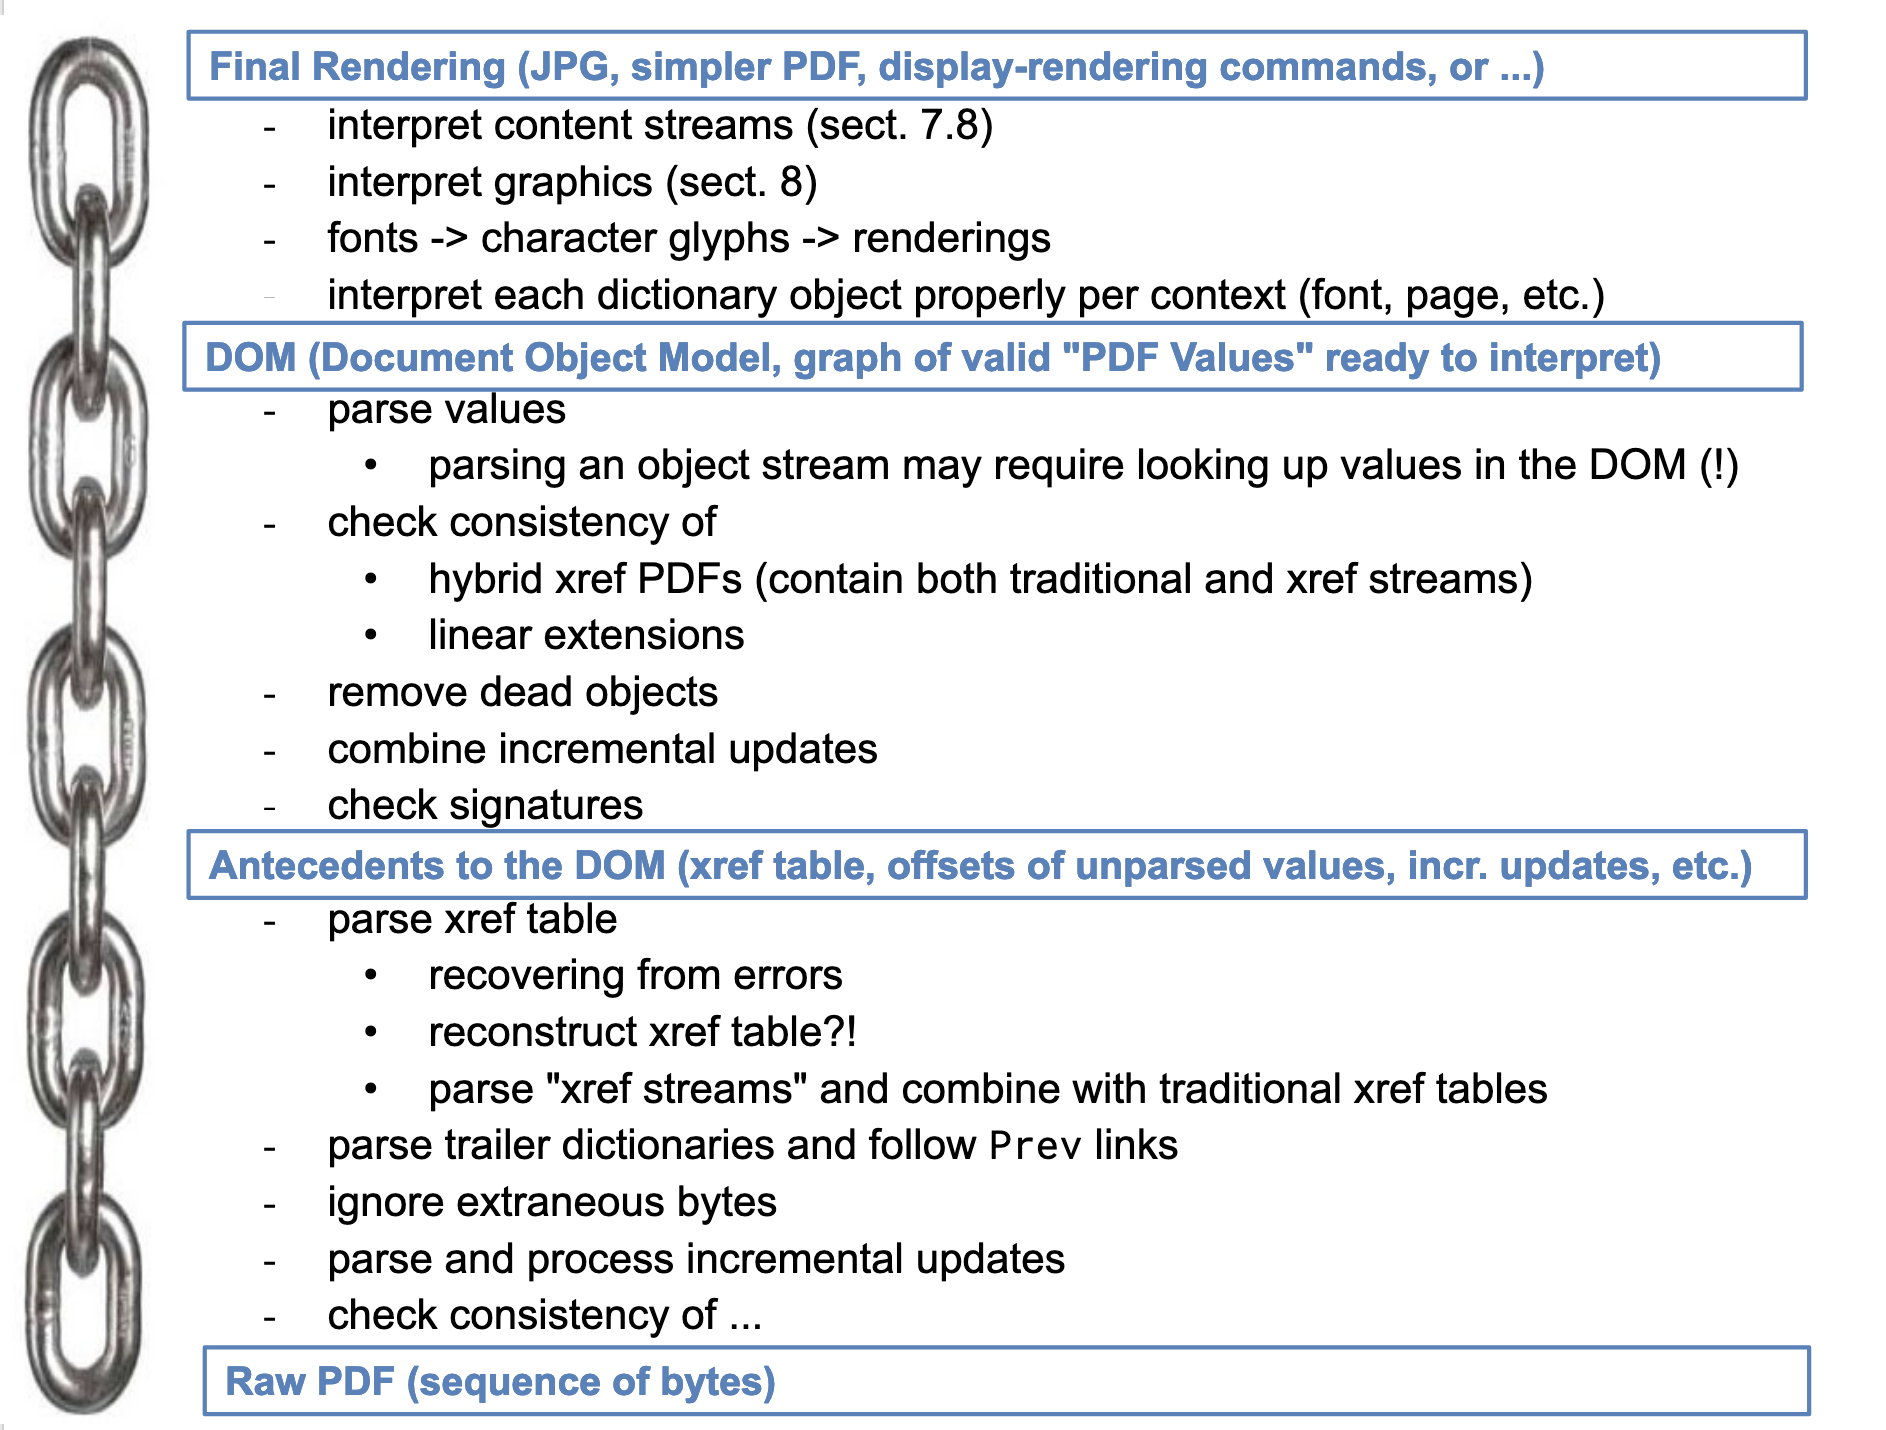
\includegraphics[width=0.8\linewidth]{figures/trustchain-diagram.png}
    \caption{The PDF Trust Chain diagrammed.}
    \todo{make diagram prettier!}
    \label{fig:pdf-trust-chain}
\end{figure}

In \cref{sec:pdf-challenges} we touched upon the complexities of parsing
PDF, but to appreciate these, one has to understand the
dependencies and interactions between the features.
In \cref{fig:pdf-trust-chain} we show the main components diagrammatically.
To briefly sketch what's going on here:
\begin{itemize}
\item Phase 1: we find the PDF header \verb|%PDF-x.y| (near start of the physical file, to account for preamble), then the end of the PDF file \verb|%%EOF| (near the end of the physical file), then "backwards parse" to find the last \verb|startxref| keyword followed by an end-of-line sequence and an integer value as ASCII bytes representing the byte offset in the PDF file (which is then adjusted for any preamble to a physical byte offset), and then locate either the \verb|xref| keyword for traditional PDF cross-reference tables, or a PDF object that should be a XRefStm stream.
  the PDF trailer (at the end of file).
\item Phase 2: using information from Phase 1, we find and parse all file
  updates.
\item Phase 3: \todo{...}
  \todo{More phases too?}
\item Phase 4: \todo{...} The result is the candidate DOM, 
  the candidate DOM is a mapping \lstcd{ObjId -> PdfValue}.
\item Phase 5: This phase takes the candidate DOM and verifies that
  it represents a sensible Document Tree per the PDF Standard.  E.g.,
  all indirect objects are in the candidate DOM, no unexpected recursion,
  etc.
\item Render Phase: we can now render the validated DOM, or parts thereof, to
  whatever display or graphic format we choose.
\end{itemize}

Note that phases 2, 3, and 4
all require inputs from the previous phase to enable them to know where and
how to parse further segments of the PDF input file.
%
Note this: an implementation \emph{might} merge phases 1-3 into single phase
and give a \emph{semblance} of simplicity, but our argument (in what
follows in \cref{sec:specifying}) is that such an implementation will be
overly complex and we will have a near unsurmountable task to assure that it
terminates for all input files.

% Only after Phase 4, have we correctly constructed a 'candidate' DOM (Document
% Object Model) where we have a mapping of Object Identifiers to PDF Values.

Although verifying Phase 5 is both difficult and tedious
(\todo{...; say something re the Arlington DOM model? Paper?})
and the Render phase has many complications of its own (fonts are
a special challenge, etc.), in this paper we focus on Phases 1-4.
We call these phases the pre-DOM parsing/computation, and if anything
goes wrong pre-DOM, lots can go wrong, the wrong DOM may be rendered, etc.!

The attentive reader will note that we have another instance of a \emph{Trust
Chain}.  The later phases of the parsing process are \emph{completely
dependent} upon the earlier phases to properly parse and interpret the PDF
file.

% The PDF "trust chain": higher levels of abstraction depend upon lower levels.
% These structures are not necessarily concrete values--e.g. parsed xref
% table--but they do exist `conceptually'.

We think it is important to understand PDF parsing in terms of this
\emph{Trust Chain} as
%
(1) it highlights the presence of the many ``dependent'' parsers (or phases)
in PDF processing.
%
(2) it highlights the importance of ensuring the pre-DOM parsing and
computation (the base of our Trust Chain) is correct and secure.
%
(3) it reminds us that the integrity of the DOM cannot be verified
independently of the lower levels.

\todo{say ... regarding our repetitious use of ``parse and compute''}
\todo{ensure that spec.hs, the above text, and \cref{sec:specifying}
      are all consistent!}

\subsection{Root Causes of PDF Complexity}

Most data formats can be described by much simpler mechanisms;
most language processors (e.g., a Python parser) can be described and parsed by
textbook methods (e.g., the old \emph{lex} and \emph{yacc} are sufficient for
most language processors);
so what makes PDF processing so much more complex?
\begin{lstlisting}[style=meta]
  - indirect offsets
    - which may recursively point to other indirect offsets
    - need programming language
      (or a 'seek' in the data definition lang)
  - DOM is a graph structure
    - objects point to objects   
  - xref tables ...
  - ... giving rise to cavities
    - giving rise to polyglots
  - dependent parsers
  - <MORE?>
\end{lstlisting}

Further detail of how these work in PDF is in \cref{sec:specifying}.

% ------------------------------------------------------------------------------
\section{Pre-DOM Vulnerabilities \note{2.5pp}}
\label{sec:predom-vulnerabilities}

As will become even more apparent, there is a significant amount of
parsing and computation that needs to be done \emph{pre-DOM}.
And given our recent points about the \emph{PDF Trust Chain}
(\cref{sec:trust-chain}),
it should not surprise us that most of the PDF attack vectors
(\cref{sec:pdf-vulnerabilities})
involve some aspect of breaking the \emph{DOM} abstraction.
I.e., they occur at the \emph{pre-DOM} levels.

{\bf{Shadow Attacks}} \todo{...}

{\bf{Schizophrenia}} \todo{...}
\begin{lstlisting}[style=meta]
  - writer errors
  - parser differentials
    - e.g., ignoring xref tables
  - recovering parsers !!
  - blind faith in incremental updates (Shadow Attacks)
\end{lstlisting}

{\bf{Polyglots}} 
\todo{... arising from cavities and permissive implementations and ...}

{\bf{Denial of Service (DOS)}} 
%
\begin{lstlisting}[style=meta]
- [potential recursion many places]
- format may not be well-defined because the recursion is not
    "well-defined"
\end{lstlisting}

{\bf{Steganography}} \todo{?}

{\bf{Others}} \todo{have any others here??}
